\documentclass[12pt]{article}  % [12pt] option for the benefit of aging markers
\usepackage{amssymb}           % amssymb package contains more mathematical symbols
\usepackage{graphicx}          % graphicx package enables you to paste graphics into your document
\usepackage{amsmath}
\usepackage{mcode}
\usepackage{float}

%%%%%%%%%%%%%%%%%%%%%%%%%%%%%%%%%
%
%    Page size commands.  Don't worry about these
%
\setlength{\textheight}{220mm}
\setlength{\topmargin}{-10mm}
\setlength{\textwidth}{150mm}
\setlength{\oddsidemargin}{0mm}

%%%%%%%%%%%%%%%%%%%%%%%%%%%%%%%%%%%%%%%%%%%%%%%%%%%%%%%%%%%%%%%
%
%    Definitions of environments for theorems etc.
%
\newtheorem{theorem}{Theorem}[section]          % Theorems numbered within sections - eg Theorem 2.1 in Section 2.
\newtheorem{corollary}[theorem]{Corollary}      % Corollaries etc. will be counted as Theorems for numbering
\newtheorem{lemma}[theorem]{Lemma}              % eg Lemma 3.1, ... Theorem 3.2, ... Corollary 3.3.
\newtheorem{proposition}[theorem]{Proposition}
\newtheorem{conjecture}[theorem]{Conjecture}

\newtheorem{definition}[theorem]{Definition}
\newtheorem{remark}[theorem]{Remark}
\newtheorem{example}[theorem]{Example} 

%--------------------------------------------------------%%%%%%%%%%%%%%%%%
%
%        Preamble material specific to your essay
%
\title{MATLAB PDE Toolbox Assignment}
\author{Cassie Hinkson\\
Boiling Water in a Campervan}

\begin{document}
\maketitle

\section{The Scenario}\label{s:intro}
%
\paragraph{} Imagine there is a person in a campervan who wishes to make a cup of tea without going outside. They have a stove with an open flame on top of a table, which they are using to boil a pot filled with water. We wish to model the change of temperature, $u(t,x,y)$, throughout the room during this process and see if these temperatures are safe for the person inside. We will do this using hyperbolic Partial Differential Equations (PDEs) solved using MATLAB's PDE Toolbox following the steps introduced in Thursday's Computer Tools and Skills lecture. 

\section{Creating the Model}
\paragraph{} To model our problem we use the hyperbolic PDE whose solution is the heat equation
\begin{equation*}
\frac{\partial u}{\partial t} \ - \ \nabla \cdot \left( c\nabla u\right) \ = \ 0.
\end{equation*}where the constant $c$, represents the conductivity of a location.
\paragraph{} We declare the model PDE as follows:

\begin{lstlisting}
numberOfPDE = 1;
pdem = createpde(numberOfPDE); %declare PDE
\end{lstlisting}

\section{The Geometry}
\paragraph{} We model the shape of the campervan and its contents by creating a geometry. The campervan and table are represented by the rectangles with coordinates $\{(1,0), (5,0), (1,2.5), (5,2.5)\}, \{(4,0), (5,0), (4,0.5), (5,0.5)\}$  respectively. The pot is modelled with the six sided polygon with coordinates $\{(4.1,0.65),(4.5,0.65),\\(4.5,0.9),(3.6,0.9),(3.6,0.87),(4.1,0.87)\}$ and the flame on the table by the ellipse centred at $(4.3;0.575)$ with width $0.1$ and height $0.14$. When creating the geometry the table is excluded since we are not concerned with how the heat spreads through it. We also exclude the flame as it is assumed to retain the same temperature throughout. The code below creates the geometry using the coordinates above.
\begin{lstlisting}
P1 = [2;6;4.1;4.5;4.5;3.6;3.6;4.1;0.65;0.65;0.9;0.9;0.87;0.87]; %pot
C1 = [3;4;1;5;5;1;0;0;2.5;2.5]; %campervan
C1 = [C1;zeros(length(P1)-length(C1),1)]; %make vector right length
T1 = [3;4;4;5;5;4;0;0;0.5;0.5];
T1 = [T1;zeros(length(P1)-length(T1),1)]; %table
H1 = [4;4.3;0.575;0.05;0.07;0]; %heat source
H1 = [H1;zeros(length(P1)-length(H1),1)];

gd=[P1,C1,T1,H1]; %includes goemetries
sf='(C1+P1)-(T1+H1)'; %doesn't include table or heat source
ns = char('P1','C1','T1','H1')';
g = decsg(gd,sf,ns); %creates geometry
\end{lstlisting}

\paragraph{} We can now plot our geometry as follows giving the plot shown in figure \ref{geom} (with the pot magnified in figure \ref{pot}).

\begin{lstlisting}
geometryFromEdges(pdem,g); 
figure %figure of geometry
pdegplot(pdem,'edgeLabels','on','subdomainLabels','on') 
axis equal
\end{lstlisting}

\begin{figure}[H]
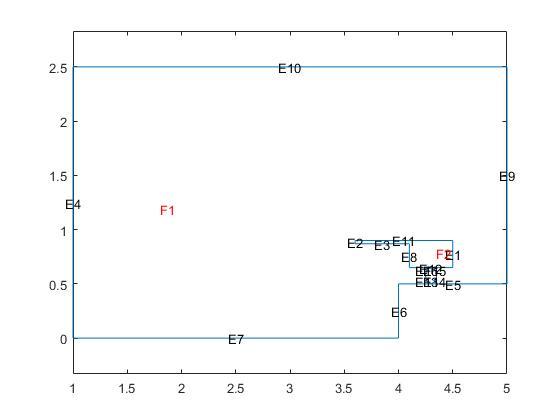
\includegraphics[scale=.75]{geometry}
\caption{Geometry of campervan}
\label{geom} 
\end{figure}
\begin{figure}[H]
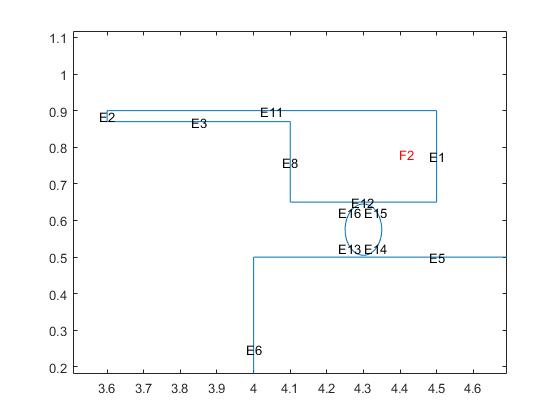
\includegraphics[scale=.5]{pot}
\caption{Magnification of pot and flame}
\label{pot}
\end{figure}

\section{Boundary and Initial Conditions}
\paragraph{} To model our problem we assume that the temperature outside the campervan is constant at 5 degrees and that the flame is constantly at 400 degrees. We reflect this in our boundary conditions by setting the temperature to be 5 on edges 4, 7, 6, 5, 9 and 10 and as 400 on edges 13, 14, 15 and 16. The campervan is assumed to be 20 degrees throughout at time $t=0$. The boundary and initial conditions are set using the code seen below.
\begin{lstlisting}
applyBoundaryCondition(pdem,'Edge',[4,7,6,5,9,10],'u',5);  %outside temp
applyBoundaryCondition(pdem,'Edge',[16,15,13,14],'u',400); %heat source temp
setInitialConditions(pdem,20); %initial room temp
\end{lstlisting}

\section{The PDE}
\paragraph{} Before solving the PDE we must define the constant $c$, the conductivity, in the different regions of the geometry. We set the conductivity as 1 for the air in the campervan (face 1) and 10 for the pot (face 2) with the code below.

\begin{lstlisting}
%set conductivity of air
specifyCoefficients(pdem,'m',0,'d',1,'c',1,'a',0,'f',0,'face',1); 
%set conductivity of pot
specifyCoefficients(pdem,'m',0,'d',1,'c',10,'a',0,'f',0,'face',2); 
\end{lstlisting}

\section{The Mesh}
\paragraph{} The code below utilizes inbuilt algorithms in MATLAB to decompose the geometry into a mesh of triangles which is optimal for solving given PDE. It also then creates a figure of the resulting mesh as seen in figure \ref{mesh}.

\begin{lstlisting}
msh = generateMesh(pdem,'Hgrad',1.05);
figure
pdemesh(pdem);
axis equal 
\end{lstlisting}

\begin{figure}[H]
	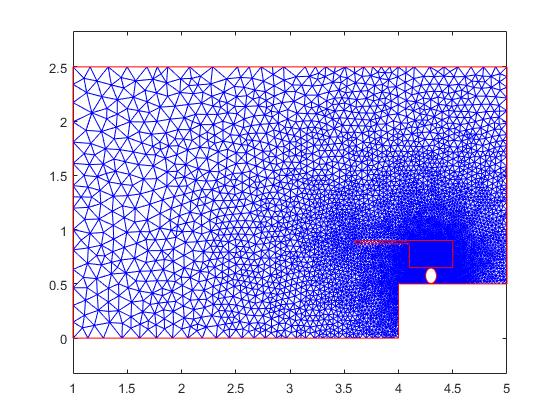
\includegraphics[scale=.75]{mesh}
	\caption{Mesh generated for geometry}
	\label{mesh}
\end{figure}

\section{The Solution}
\paragraph{} The solution, $u(t,x,y)$, of our PDE is obtained by creating an array of 200 time steps in the interval $(0,0.1)$ and then solving the PDE at all steps. A movie is then created by saving heat maps taken at each time step. We are particularly interested in the temperature of our model for all $t\in(0,0.1)$ at three locations: inside the pot where water would be, the handle of the pot and in a position near the pot where a person would stand, possibly holding the handle of the pot. These points are taken to be $(4.25,0.7), (3.7,0.88)$ and $(3.25,1.25)$ respectively. We then interpolate our solution at these three points and create a plot to show the temperature at them over time. The above is performed using the code below resulting in the subsequent figures \ref{3point} and \ref{heatmap}.

\begin{lstlisting}
nframes = 200; %# time steps in soln
tlist = linspace(0,0.1,nframes);
pdem.SolverOptions.ReportStatistics ='on'; %check soln is good
result = solvepde(pdem,tlist); %solves PDE
u1 = result.NodalSolution;

%points to follow temp change - in pot, handle, standing pos for person
xx = [4.25,3.7,3.25];
yy = [0.7,0.88,1.25];
uintrp = interpolateSolution(result,xx,yy,1:length(tlist));

figure
for j= 1:3
hold on
plot(tlist,uintrp(j,:))
hold off
end
title('Change of T over time at three points')
xlabel('time')
ylabel('temperature')
legend('pot','handle','person')

figure 
for j = 1:nframes, pdeplot(pdem,'xydata',u1(:,j),'colormap','hot');
hold on 
pdegplot(pdem);
hold off 
Mv(j) = getframe;
end
movie(Mv,1);

\end{lstlisting}

\begin{figure}[H]
	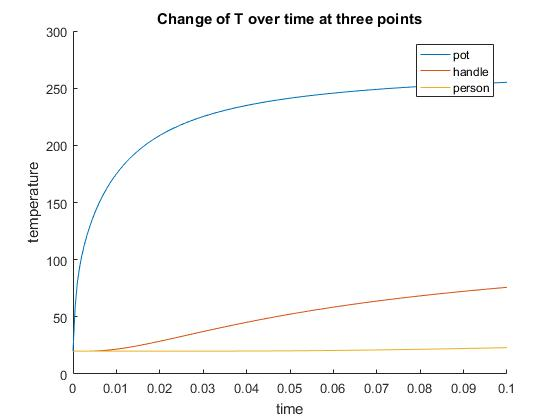
\includegraphics[scale=.75]{3pointplot}
	\caption{Temperature at 3 points for $t=[0,0.1]$}
	\label{3point}
\end{figure}
\begin{figure}[H]
	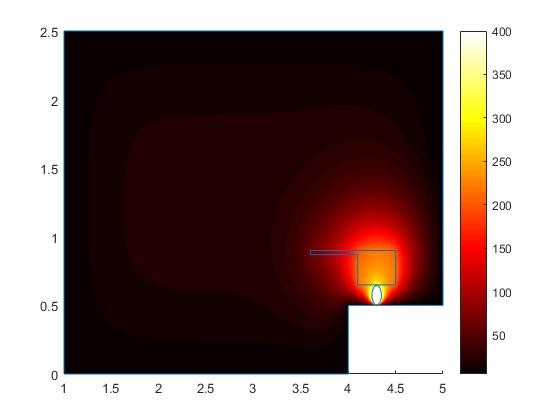
\includegraphics[scale=.75]{heatmap}
	\caption{Heat map at $t=0.1$}
	\label{heatmap}
\end{figure}
\section{The Steady State}
\paragraph{} If we were to leave our model of the pot on the flame for a long time, it would eventually reach a steady state where the temperature would not change over time ($u(t_h,x,y)=u(t_{h+1},x,y)$ where $h,h+1$ are time steps taken after the system reaches its steady state). 
We can find the solution $u$ for the steady state by altering the hyperbolic PDE solved above, we do this by changing the coefficient, $d$ of the term $\frac{\partial u}{\partial t}$ from 1 to 0, reflecting how the new solution is unchanging in time. We also remove the initial condition used above as our solution is now only dependant on position in space.
Below the new coefficients are specified followed by the code used to generate our new solution at the three points and heat map of the steady state (figure \ref{heatmap2}). 

\begin{lstlisting}
%set conductivity of air
specifyCoefficients(pdem1,'m',0,'d',0,'c',1,'a',0,'f',0,'face',1);
%set conductivity of pot 
specifyCoefficients(pdem1,'m',0,'d',0,'c',10,'a',0,'f',0,'face',2);

result = solvepde(pdem1);
u1 = result.NodalSolution;

%points to assess temp at - in pot, handle, standing pos for person
xx = [4.25,3.7,3.25];
yy = [0.7,0.88,1.25];
uintrp = interpolateSolution(result,xx,yy);
uintrp

figure 
pdeplot(pdem1,'xydata',u1,'colormap','hot'); 
hold on 
pdegplot(pdem1);
hold off 

\end{lstlisting}

\begin{figure}[H]
	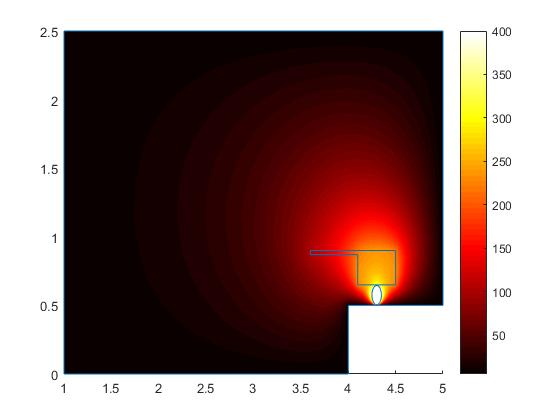
\includegraphics[scale=.75]{heatmap2}
	\caption{Heat map of steady state}
	\label{heatmap2}
\end{figure}

The steady state temperatures for inside the pot, the handle and where a person may stand are given respectively as the output for 'uintrp':

\begin{lstlisting}
uintrp =

267.9281
116.4851
54.4852
\end{lstlisting}


\section{Conclusion}
\paragraph{} Figure \ref{3point} obtained in section 7 shows that over the time interval the temperature of the pot reaches over 250 degrees, so water in the pot would be expected to reach boiling point given enough time. However the model uses a cross section of all one material when in reality we would have a metal handle and hollow pot with most of the cross section being made up of water. To make the model more realistic we could add the water into the cross section of the pot. As expected the handle of the pot gets hot and reaches around 75 degrees, which is approaching the temperature when one would need to use a glove to hold it. The temperature for a person standing near by is only slightly increased and wouldn't cause them any discomfort.
\paragraph{}In the steady state model we find that the pot temperature reaches only a little hotter than in the first solution. The handle temperature is now definitely too hot to hold without protection. The temperature for someone standing by the pot is approaching that of record breaking desert-like conditions and would most likely be intolerable to someone used to living in Britain. This result is quite surprising and seems like it could be inaccurate due to the constant boundary conditions used. We could probably obtain a more realistic solution using flux boundary conditions in future attempts.



%%%%%%%%%%%%%%%%%%%%%%%%%%%%%%%%%%%%%%%%%
%
%     Bibliography
%
%     Use an easy-to-remember tag for each entry - eg \bibitem{How97} for an article/book by Howie in 1997
%     To cite this publication in your text, write \cite{How97}.  To include more details such as
%     page, Chapter, Theorem numbers, use the form \cite[Theorem 6.3, page 42]{How97}.
%

\end{document}
